% --------------------------------------------------------------
% This is all preamble stuff that you don't have to worry about.
% Head down to where it says "Start here"
% --------------------------------------------------------------
 
\documentclass[12pt]{article}
 
\usepackage[margin=1in]{geometry} 
\usepackage{amsmath,amsthm,amssymb}
\usepackage[T1]{fontenc}
\usepackage{graphicx} %package to manage images
\graphicspath{ {images/} }
\usepackage[rightcaption]{sidecap}
\usepackage{wrapfig}

 
\newcommand{\N}{\mathbb{N}}
\newcommand{\Z}{\mathbb{Z}}
 
\newenvironment{theorem}[2][Theorem]{\begin{trivlist}
\item[\hskip \labelsep {\bfseries #1}\hskip \labelsep {\bfseries #2.}]}{\end{trivlist}}
\newenvironment{lemma}[2][Lemma]{\begin{trivlist}
\item[\hskip \labelsep {\bfseries #1}\hskip \labelsep {\bfseries #2.}]}{\end{trivlist}}
\newenvironment{exercise}[2][Exercise]{\begin{trivlist}
\item[\hskip \labelsep {\bfseries #1}\hskip \labelsep {\bfseries #2.}]}{\end{trivlist}}
\newenvironment{reflection}[2][Reflection]{\begin{trivlist}
\item[\hskip \labelsep {\bfseries #1}\hskip \labelsep {\bfseries #2.}]}{\end{trivlist}}
\newenvironment{proposition}[2][Proposition]{\begin{trivlist}
\item[\hskip \labelsep {\bfseries #1}\hskip \labelsep {\bfseries #2.}]}{\end{trivlist}}
\newenvironment{corollary}[2][Corollary]{\begin{trivlist}
\item[\hskip \labelsep {\bfseries #1}\hskip \labelsep {\bfseries #2.}]}{\end{trivlist}}
\newenvironment{problem}[2][Problem]{\begin{trivlist}
\item[\hskip \labelsep {\bfseries #1}\hskip \labelsep {\bfseries #2.}]}{\end{trivlist}}
 
\begin{document}

\topmargin=-0.45in
\evensidemargin=0in
\oddsidemargin=0in
\textwidth=6.5in
\textheight=9.0in
\headsep=0.25in 
 
% --------------------------------------------------------------
%                         Start here
% --------------------------------------------------------------
 
%\renewcommand{\qedsymbol}{\filledbox}
 
\title{CSCI 567: Homework 3}%replace X with the appropriate number
\author{Deepika Anand} %replace with your name
\maketitle

\begin{problem} 2 (a)
\end{problem}
\begin{Answer}
For any function F(.) if K is valid kernel then, 
\begin{equation}
    \int_{x, x'} f(x) f(x') k(x, x') dx dx' >= 0
\end{equation}
So, $k_{3}$ can be replaced with $a_{1}k_{1} + a_{2}k_{2}$\\
\begin{equation}
    \int_{x, x'} f(x) f(x') [ a_{1}k_{1}(x.x') + a_{2}k_{2}(x.x')] dx dx'
\end{equation}
this can be rewritten as 
\begin{equation}
    \int_{x, x'} f(x) f(x') [ a_{1}k_{1}(x.x') ] dx dx' + \int_{x, x'} f(x) f(x') [ a_{2}k_{2}(x.x')] dx dx'
\end{equation}
Since both the component are greater than zero so the addition of the two will be greater than 0, hence we can write $k_{3}$ is valid
\end{Answer}

\begin{problem} 2 (b)
\end{problem}
\begin{Answer}
As $k_{4}$ can be written as NXN matrix for the points f($x_{1}$).....f($x_{n}$)\\
$k_{4} = V^{T} F F^{T} V$\\
Now combing terms it can be written as
$k_{4} = (F^{T}V)^{T} F^{T} V$\\
or $k_{4} = || F^{T} V||^2$\\
Since square of a scalar quantity is always greater than 0. Hence $k_{4}$ is valid kernel
\end{Answer}

\begin{problem} 2 (c)
\end{problem}
\begin{Answer}
As stated in part (a) that if K is kernel it can be written as\\
\begin{equation}
    \int_{x, x'} f(x) f(x') k(x, x') dx dx' >= 0
\end{equation}
Since in this case both $k_{1}$ and $k_{2}$ are valid kernels. Hence\\
\begin{equation}
    \int_{x, x'} f(x) f(x') k_{1}(x, x') dx dx' >= 0
\end{equation}\\
and 
\begin{equation}
    \int_{x, x'} f(x) f(x') k_{2}(x, x') dx dx' >= 0
\end{equation}
Hence, product of two will also be greater than 0. Hence, multiplying them we get\\
\begin{equation}
    \int_{x, x'} f(x) f(x') k_{1}(x, x') dx dx' * \int_{x, x'} f(x) f(x') k_{2}(x, x') dx dx' >= 0
\end{equation}
Hence $k_{5}$ is a valid kernel.
\end{Answer}

\begin{problem} 4 (a)
\end{problem}
\begin{Answer}
No, the data is not linearly separable
\end{Answer}

\begin{problem} 4 (b)
\end{problem}
\begin{Answer}
The data is not linearly separable in 2D plane but when projected to higher dimension there will be a hyperplane which will be able to separate them. That hyperplane when projected to 2D space will by a quadratic curve. Hence we need to assign weightage such that $x_{1}x_{2}$ = 1. \\
Hence W = [ 0 0 0 1 ]
\end{Answer}

\begin{problem} 4 (c)
\end{problem}
\begin{Answer}
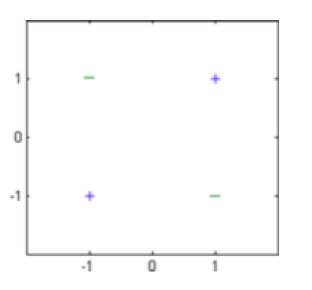
\includegraphics{Problem4}
\end{Answer}

\begin{problem} 4 (d)
\end{problem}
\begin{Answer}
K = \Phi(x)\Phi(x')\\
$\Phi(x) = [ 1 \hskip 1em x_{1} \hskip 1em x_{2} \hskip 1em x_{1}x_{2} ]$\\
$\Phi(x') = [ 1 \hskip 1em x_{1}' \hskip 1em  x_{2}' \hskip 1em x_{1}'x_{2}' ]$\\
Taking Transpose of $\Phi(x)$ and then multiplying with $\Phi(x')$\\
We get feature transformation, $[1 \hskip 1em x_{1}x_{1}' \hskip 1em x_{2}x_{2}' \hskip 1em x_{1}x_{1}'x_{2}x_{2}']$
\end{Answer}

\begin{problem} 5 (a)
\end{problem}
\begin{Answer}
The error function J is given as 
\begin{equation}
    J = ||w|| ^ 2 + C \sum_{i=1}^{N} e_{n} 
\end{equation}
such that $y_{n}(w^{T}x_{n} + b) >= 1 - e_{n}$ for n = 1, 2.....N\\
For large values of C, penalizing shrinking the margin heavily. This means decision boundary will separate the data perfectly.
\end{Answer}


\begin{problem} 5 (b)
\end{problem}
\begin{Answer}
C = 0, some $e_{n}$ is allowed that is some misclassification is not penalised heavily while maximizing the margin between the points
\end{Answer}

\begin{problem} 5 (c)
\end{problem}
\begin{Answer}
As mentioned in the problem statement itself that "avoid trusting any data point too much". Hence, we chose the case when C ~ 0
\end{Answer}

\begin{problem} 5 (d)
\end{problem}
\begin{Answer}
Marking the point which would have been correctly identified by the classifier and hence will not be a support vector.
\end{Answer}

\begin{problem} 5 (e)
\end{problem}
\begin{Answer}
Since C is very large therefore misclassifying a single data point will involve huge penalty and hence the boundary will move significantly.
\end{Answer}
\begin{figure}
    \advance\leftskip-1cm
    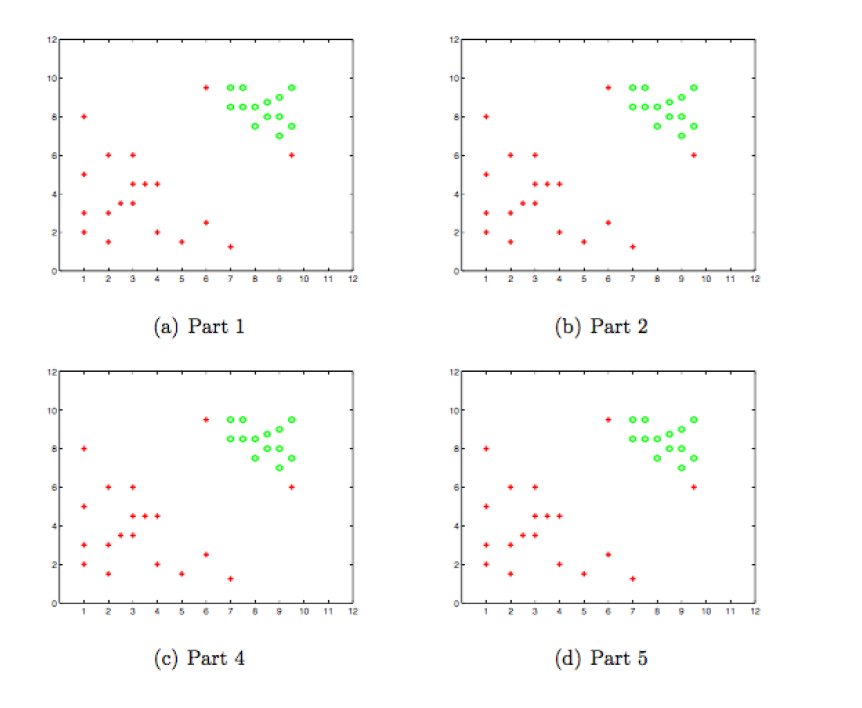
\includegraphics[options]{Problem5}
\end{figure}

\clearpage
\begin{problem} 6 (a) (i)
\end{problem}
\begin{Answer}
With 100 datasets 10 samples each
\begin{verbatim}
     Function     Bias2     Variance
     g1(x)        0.465     0.000
     g2(x)        0.338     0.605
     g3(x)        0.284     0.612
     g4(x)        0.028     0.643
     g5(x)        0.038     0.644
     g6(x)        0.051     0.645
\end{verbatim}
\end{Answer}

\begin{problem} 6 (a) (ii)
\end{problem}
\begin{Answer}
With 100 datasets 100 samples each
\begin{verbatim}
     Function     Bias2     Variance
     g1(x)        0.469     0.000
     g2(x)        0.350     0.000
     g3(x)        0.346     0.007
     g4(x)        0.003     0.350
     g5(x)        0.004     0.351
     g6(x)        0.005     0.352
\end{verbatim}
\end{Answer}

\begin{problem} 6 (a) (iii)
\end{problem}
\begin{Answer}
\textbf{Model Complexity impact on bias and variance}\\
As clear from the results. Model complexity has a strong impact on both bias and variance. When complexity is low then bias is high but variance is low however as gradually increase complexity from $g_{1}(x)$ to $g_{6}(x)$ then bias decreases but variance increased. Hence, there is always a tradeoff between best value of bias and variance. \\

\textbf{Sample Size impact on bias and variance }
The results show that there is not much difference in the values of bias squared and variance with size of data set. Hence, we can say the bias square or bias itself and variance are independent of sample size/data points
\end{Answer}

\begin{problem} 6 (a) (iv)
\end{problem}
\begin{Answer}
\begin{verbatim}
     lambda  bias2    variance
     0.001   0.003    0.345
     0.003   0.003    0.345
     0.010   0.005    0.347
     0.030   0.018    0.360
     0.100   0.164    0.506
     0.300   1.437    1.779
     1.000   15.880   16.223
\end{verbatim}
$\lambda$ is the regularizer used to prevent overfitting. Hence as lambda increases we see that both bias square and variance increased. However it can be seen that bias increases polynomially whereas variance increases exponentially.
\end{Answer}

\begin{problem} 6 (b) (i)
\end{problem}
\begin{Answer}
\textbf{Linear SVM}\\ 
    \begin{tabular}{lll}
    C        & Time     & Accuracy \\ 
    0.000244 & 1056.600 & 55.75\%  \\
    0.000977 & 1040.189 & 87.80\%  \\
    0.003906 & 689.316  & 91.30\%  \\
    0.015625 & 482.268  & 92.40\%  \\
    0.0625   & 360.110  & 93.70\%  \\
    0.25     & 311.735  & 94.60\%  \\
    1        & 305.660  & 94.20\%  \\
    4        & 336.019  & 94.70\%  \\
    16       & 503.622  & 94.50\%  \\ 
    \end{tabular}\\

Linear SVM Average Time taken = 565.058 ms\\
\end{Answer}

\begin{problem} 6 (b) (ii)
\end{problem}
\begin{Answer}
\textbf{Polynomical SVM}\\ 
\begin{tabular}{llll}
C        & Degree & Time     & Accuracy \\
0.015625 & 1      & 1011.962 & 55.75\%  \\
0.015625 & 2      & 1016.618 & 55.75\%  \\
0.015625 & 3      & 1040.559 & 55.75\%  \\
0.0625   & 1      & 908.06   & 88.45\%  \\
0.0625   & 2      & 952.376  & 88.00\%  \\
0.0625   & 3      & 1002.274 & 76.05\%  \\
0.25     & 1      & 599.397  & 91.70\%  \\
0.25     & 2      & 676.934  & 91.40\%  \\
0.25     & 3      & 750.08   & 91.35\%  \\
1        & 1      & 402.76   & 92.35\%  \\
1        & 2      & 441.698  & 92.75\%  \\
1        & 3      & 556.058  & 92.55\%  \\
4        & 1      & 342.307  & 94.10\%  \\
4        & 2      & 320.912  & 94.45\%  \\
4        & 3      & 418.816  & 94.95\%  \\
16       & 1      & 299.481  & 94.20\%  \\
16       & 2      & 292.204  & 95.40\%  \\
16       & 3      & 304.433  & 95.15\%  \\
64       & 1      & 295.741  & 94.55\%  \\
64       & 2      & 280.27   & 96.45\%  \\
64       & 3      & 296.836  & 96.50\%  \\
256      & 1      & 366.073  & 94.75\%  \\
256      & 2      & 285.051  & 96.00\%  \\
256      & 3      & 295.968  & 95.60\%  \\
1024     & 1      & 712.163  & 94.30\%  \\
1024     & 2      & 311.094  & 96.10\%  \\
1024     & 3      & 300.126  & 96.15\%  \\
4096     & 1      & 3053.702 & 94.60\%  \\
4096     & 2      & 348.923  & 96.10\%  \\
4096     & 3      & 332.564  & 96.25\%  \\
16384    & 1      & 8054.946 & 94.70\%  \\
16384    & 2      & 396.205  & 94.75\%  \\
16384    & 3      & 320.804  & 96.15\% 
\end{tabular}\\
Polynomial SVM Average Time taken = 817.799 ms\\
\end{Answer}

\clearpage

\begin{problem} 6 (b) (iii)
\end{problem}
\begin{Answer}
\textbf{RBF SVM}\\ 
\begin{table}[]
\begin{tabular}{llll}
C        & Gamma       & Time     & Accuracy \\
0.015625 & 6.10E-05    & 1061.8   & 55.75\%  \\
0.015625 & 0.000244141 & 1050.42  & 55.75\%  \\
0.015625 & 0.000976563 & 1047.517 & 55.75\%  \\
0.015625 & 0.00390625  & 1078.563 & 55.75\%  \\
0.015625 & 0.015625    & 1063.569 & 55.75\%  \\
0.015625 & 0.0625      & 1053.215 & 85.05\%  \\
0.015625 & 0.25        & 1070.264 & 64.85\%  \\
0.0625   & 6.10E-05    & 1043.1   & 55.75\%  \\
0.0625   & 0.000244141 & 1038.406 & 55.75\%  \\
0.0625   & 0.000976563 & 1051.154 & 55.75\%  \\
0.0625   & 0.00390625  & 1066.258 & 56.35\%  \\
0.0625   & 0.015625    & 927.338  & 88.25\%  \\
0.0625   & 0.0625      & 734.682  & 91.75\%  \\
0.0625   & 0.25        & 904.228  & 88.35\%  \\
0.25     & 6.10E-05    & 1074.592 & 55.75\%  \\
0.25     & 0.000244141 & 1037.26  & 55.75\%  \\
0.25     & 0.000976563 & 1129.653 & 57.80\%  \\
0.25     & 0.00390625  & 857.931  & 88.75\%  \\
0.25     & 0.015625    & 610.535  & 91.60\%  \\
0.25     & 0.0625      & 481.26   & 93.25\%  \\
0.25     & 0.25        & 620.225  & 95.85\%  \\
1        & 6.10E-05    & 1050.266 & 55.75\%  \\
1        & 0.000244141 & 1064.237 & 58.40\%  \\
1        & 0.000976563 & 857.085  & 88.95\%  \\
1        & 0.00390625  & 569.983  & 91.70\%  \\
1        & 0.015625    & 429.599  & 93.00\%  \\
1        & 0.0625      & 365.589  & 95.40\%  \\
1        & 0.25        & 452.834  & 96.60\%  \\
4        & 6.10E-05    & 1102.983 & 58.05\%  \\
4        & 0.000244141 & 856.415  & 88.90\%  \\
4        & 0.000976563 & 543.146  & 91.60\%  \\
4        & 0.00390625  & 413.173  & 92.80\%  \\
4        & 0.015625    & 317.382  & 95.10\%  \\
4        & 0.0625      & 309.27   & 96.15\%  \\
4        & 0.25        & 414.182  & 97.05\%  \\
16       & 6.10E-05    & 845.231  & 88.80\%  \\
16       & 0.000244141 & 561.33   & 92.05\%  \\
16       & 0.000976563 & 398.042  & 93.15\%  \\
16       & 0.00390625  & 330.384  & 94.50\%  \\
16       & 0.015625    & 310.161  & 94.70\%  \\
16       & 0.0625      & 284.351  & 97.30\%  \\
16       & 0.25        & 423.867  & 96.90\%  \\
64       & 6.10E-05    & 581.785  & 91.65\%  \\
64       & 0.000244141 & 395.415  & 92.90\%  \\
64       & 0.000976563 & 333.241  & 94.40\%  \\
64       & 0.00390625  & 294.86   & 94.60\%  \\
64       & 0.015625    & 298.986  & 96.05\%  \\

\end{tabular}
\end{table}\\
\clearpage

\begin{table}
\begin{tabular}{llll}
C        & Degree & Time     & Accuracy \\
64       & 0.0625      & 251.185  & 96.15\%  \\
64       & 0.25        & 407.012  & 96.30\%  \\
256   & 6.10E-05    & 405.13  & 92.90\% \\
256   & 0.000244141 & 342.399 & 94.70\% \\
256   & 0.000976563 & 301.386 & 94.75\% \\
256   & 0.00390625  & 307.522 & 95.00\% \\
256   & 0.015625    & 297.893 & 96.15\% \\
256   & 0.0625      & 278.306 & 95.80\% \\
256   & 0.25        & 422.788 & 96.60\% \\
1024  & 6.10E-05    & 338.111 & 94.40\% \\
1024  & 0.000244141 & 311.198 & 93.95\% \\
1024  & 0.000976563 & 289.898 & 95.10\% \\
1024  & 0.00390625  & 328.884 & 95.95\% \\
1024  & 0.015625    & 324.54  & 96.45\% \\
1024  & 0.0625      & 272.482 & 96.40\% \\
1024  & 0.25        & 398.502 & 96.30\% \\
4096  & 6.10E-05    & 314.339 & 94.50\% \\
4096  & 0.000244141 & 303.496 & 94.35\% \\
4096  & 0.000976563 & 350.254 & 94.75\% \\
4096  & 0.00390625  & 398.03  & 96.30\% \\
4096  & 0.015625    & 334.979 & 96.25\% \\
4096  & 0.0625      & 287.481 & 96.55\% \\
4096  & 0.25        & 420.431 & 96.50\% \\
16384 & 6.10E-05    & 319.362 & 94.40\% \\
16384 & 0.000244141 & 364.48  & 95.05\% \\
16384 & 0.000976563 & 511.049 & 96.35\% \\
16384 & 0.00390625  & 495.711 & 96.45\% \\
16384 & 0.015625    & 392.41  & 96.80\% \\
16384 & 0.0625      & 279.571 & 96.20\% \\
16384 & 0.25        & 399.651 & 96.40\%
\end{tabular}
\end{table}
RBF SVM Average Time taken = 574.730 ms\\
\end{Answer}

\begin{problem} 6 (b) (iv)
\end{problem}
\begin{Answer}
Selected RBF Kernel with C = 16384 that is $4^{7}$ and gamma = 0.015625 that is $4^{-3}$ \\
Accuracy = 95.55$\%$  \\
Number of correct prediction/Size of test    data = (1911/2000)
\end{Answer}


\end{document}

